\documentclass[a4paper, 12pt, journal]{ieeeconf}\usepackage[]{graphicx}\usepackage[]{color}
%% maxwidth is the original width if it is less than linewidth
%% otherwise use linewidth (to make sure the graphics do not exceed the margin)
\makeatletter
\def\maxwidth{ %
  \ifdim\Gin@nat@width>\linewidth
    \linewidth
  \else
    \Gin@nat@width
  \fi
}
\makeatother

\definecolor{fgcolor}{rgb}{0.345, 0.345, 0.345}
\newcommand{\hlnum}[1]{\textcolor[rgb]{0.686,0.059,0.569}{#1}}%
\newcommand{\hlstr}[1]{\textcolor[rgb]{0.192,0.494,0.8}{#1}}%
\newcommand{\hlcom}[1]{\textcolor[rgb]{0.678,0.584,0.686}{\textit{#1}}}%
\newcommand{\hlopt}[1]{\textcolor[rgb]{0,0,0}{#1}}%
\newcommand{\hlstd}[1]{\textcolor[rgb]{0.345,0.345,0.345}{#1}}%
\newcommand{\hlkwa}[1]{\textcolor[rgb]{0.161,0.373,0.58}{\textbf{#1}}}%
\newcommand{\hlkwb}[1]{\textcolor[rgb]{0.69,0.353,0.396}{#1}}%
\newcommand{\hlkwc}[1]{\textcolor[rgb]{0.333,0.667,0.333}{#1}}%
\newcommand{\hlkwd}[1]{\textcolor[rgb]{0.737,0.353,0.396}{\textbf{#1}}}%
\let\hlipl\hlkwb

\usepackage{framed}
\makeatletter
\newenvironment{kframe}{%
 \def\at@end@of@kframe{}%
 \ifinner\ifhmode%
  \def\at@end@of@kframe{\end{minipage}}%
  \begin{minipage}{\columnwidth}%
 \fi\fi%
 \def\FrameCommand##1{\hskip\@totalleftmargin \hskip-\fboxsep
 \colorbox{shadecolor}{##1}\hskip-\fboxsep
     % There is no \\@totalrightmargin, so:
     \hskip-\linewidth \hskip-\@totalleftmargin \hskip\columnwidth}%
 \MakeFramed {\advance\hsize-\width
   \@totalleftmargin\z@ \linewidth\hsize
   \@setminipage}}%
 {\par\unskip\endMakeFramed%
 \at@end@of@kframe}
\makeatother

\definecolor{shadecolor}{rgb}{.97, .97, .97}
\definecolor{messagecolor}{rgb}{0, 0, 0}
\definecolor{warningcolor}{rgb}{1, 0, 1}
\definecolor{errorcolor}{rgb}{1, 0, 0}
\newenvironment{knitrout}{}{} % an empty environment to be redefined in TeX

\usepackage{alltt}  
\usepackage{cite}

\overrideIEEEmargins

\title{\LARGE \bf
Homogeneously-Mixed Models versus Heterogeneously-Mixed Models in Pandemic Influenza Epidemics
}

\author{Alexandra Bushby$^{1}$, Alexei Kuzmin$^{2}$, Claudia Tugulan$^{3}$, Roger Zhang$^{4}$% <-this % stops a space
}
%% page layout
\textheight 9in 
\textwidth 6.5in
\topmargin -0.5in
\oddsidemargin 0in
\evensidemargin 0in
%\hoffset=-0.5in
\voffset=-0.25in

%% packages
\usepackage{scrtime} % for \thistime (this package MUST be listed first!)
\usepackage{amsmath} % essential for cases environment
\usepackage{amsthm} % for theorems and proofs
\usepackage{amsfonts} % mathbb
\usepackage{graphics,graphicx}
\usepackage{multirow} % fancy tables
\usepackage{wasysym} % circle symbols (including half-filled circles)
\usepackage{enumerate} % fancier enumeration (e.g., a,b,c, ...)
%\usepackage{IEEEtrantools}
\usepackage[]{float}
%\usepackage{xcolor}
\usepackage{color}
\newcommand{\de}[1]{{\color{red}{\bfseries DE:} #1}}
\newcommand{\ab}[1]{{\color{blue}{\bfseries AB:} #1}}


%% for solutions to multiple choice questions:
\newcommand{\correct}{{\color{blue}\fbox{\color{red}\checkmark} }}

%% macros
\newcommand{\reals}{\mathbb{R}}
\newcommand{\term}[1]{{\bfseries\slshape #1}}
\newcommand{\Ker}{{\text{Ker}\,}}
\newcommand{\Range}{{\text{Range}\,}}
\newcommand{\diag}{{\text{diag}}}
\newcommand{\alg}{{\text{alg}}}
\newcommand{\geom}{{\text{geom}}}
\newcommand{\norm}[1]{\left\|#1\right\|}
\newcommand{\abs}[1]{\left|#1\right|}
\newcommand{\R}{{\cal R}}
\newcommand{\G}{{\cal G}}
\newcommand{\eps}{\varepsilon}
\newcommand{\B}{\cal B}
\newcommand{\Tinf}{T_\textrm{inf}}
\newcommand{\Shat}{{\hat{S}}}
\newcommand{\Ihat}{{\hat{I}}}
\newcommand{\ie}{\emph{i.e., }}
\newcommand{\eg}{\emph{e.g., }}
\newcommand{\Rlogo}{\protect
\includegraphics[height=2ex,keepaspectratio]{images/Rlogo.pdf}\xspace}
\newcommand{\XPPAUT}{\texttt{XPPAUT}\xspace}
\newcommand{\etal}{\textit{et al}.\xspace}
\newcommand\emphblue[1]{\emph{\color{blue}#1}}

%%%%%%%%%%%%%%%%%%%%%%%%%%%%
%% from feverpreamble.tex %%
%%%%%%%%%%%%%%%%%%%%%%%%%%%%

\usepackage{amssymb,latexsym,amsmath,setspace}
%%\usepackage[colorlinks,linkcolor=blue]{hyperref}
\usepackage[colorlinks=true,allcolors=blue]{hyperref}
%%\usepackage[colorlinks]{hyperref}
\usepackage{xspace}
\usepackage{graphics,graphicx}
\usepackage{subfigure}
\usepackage{lineno}
\usepackage{fancyhdr}
\usepackage[english]{babel}  %% for texi2dvi ~ bug
\usepackage[normalem]{ulem}
\usepackage{tikz} % http://www.texample.net/tikz/examples/tikzdevice-demo/
  % N.B. version 0.6.3 of tikzDevice from Rforge is required!!
%% improve figure caption typsetting:  (see ~/tex/caption.pdf for manual)
\usepackage[footnotesize,bf]{caption}
\usepackage{placeins} % \FloatBarrier

\usepackage{tikz}
\usetikzlibrary{shapes,arrows}
\usepackage{amsmath,bm,times}
\usepackage{filecontents}
\tikzstyle{susceptible}=[draw, fill=blue!20, text width=5em, 
    text centered, minimum height=2.5em, rounded corners]
\tikzstyle{infectious}=[draw, fill=red!20, text width=5em, 
    text centered, minimum height=2.5em, rounded corners]
\tikzstyle{ann} = [above, text width=5em]
\tikzstyle{removed} = [susceptible, text width=5em, fill=green!20, 
    minimum height=2.5em, rounded corners]

% citation macros
%%\newcommand{\citen}[1]{\cite{#1}}

% comment macros
\usepackage{color}
\newcommand{\comment}[3]{\textcolor{#1}{\textbf{[#2: }\textit{#3}\textbf{]}}}
\newcommand{\alex}[1]{\comment{blue}{AB}{#1}}
\newcommand{\roger}[1]{\comment{brown}{RZ}{#1}}
\newcommand{\claudia}[1]{\comment{cyan}{CT}{#1}}
\newcommand{\alexei}[1]{\comment{magenta}{AK}{#1}}
\newcommand{\needref}{{\textcolor{red}{[NEED REF]}}}
\newcommand{\TBD}{{\textcolor{red}{{\bf TBD}}}}
% remove comments
%\renewcommand{\comment}[3]{\relax}
% remove section headings
%\def\subsubsection*#1{\relax\nobreak}

% other macros
\newcommand{\avg}[1]{{\left\langle#1\right\rangle}}
\newcommand{\var}[1]{\textrm{var}\left(#1\right)}
\newcommand{\sem}[1]{\textrm{sem}\left(#1\right)}
\newcommand{\natinf}{{\mathcal I}}
\newcommand{\find}{f_{\textrm{i}}}
\newcommand{\fpop}{f_{\textrm{p}}}
\newcommand{\logit}{\textrm{logit}}
\newcommand{\sign}{\textrm{sign}}
\newcommand{\logistic}{\textrm{logistic}}
\def\AJE{{\it American Journal of Epidemiology\/}}
\newcommand{\code}[1]{{\tt #1}}
\newcommand{\magcode}[1]{{\tt\color{magenta}#1}}
\newcommand{\redcode}[1]{{\tt\color{red}#1}}
\newcommand{\blackcode}[1]{{\tt\color{black}#1}}

%%%%%%%%%%%%%%%%%%%
%% JOURNAL NAMES %%
%%%%%%%%%%%%%%%%%%%
\def\PNAS{PNAS}
\def\JAMA{JAMA}
\def\BMB{{\it Bulletin of Mathematical Biology\/}}

% references
\newcommand{\eref}[1]{Equation~\eqref{E:#1}}
\newcommand{\fref}[1]{Figure~\ref{F:#1}}
\newcommand{\tref}[1]{Table~\ref{T:#1}}
\newcommand{\sref}[1]{\S\ref{S:#1}}
% other macros
\newcommand{{\Reff}}{{\mathcal{R}}_{\rm eff}}
\newcommand{{\Sinit}}{S_{\rm init}}
\newcommand{\supp}{Supplementary Information}
\newcommand{\StoppedHere}{\bigskip\bigskip{\textcolor{red}{\hrule\centerline{\bfseries STOPPED HERE}\hrule}}\bigskip\bigskip}
\newcommand{\colvec}[2]{\begin{pmatrix}#1\\#2\end{pmatrix}}
\newcommand{\diagmat}[3]{\begin{pmatrix}#1&0&0\\0&#2&0\\0&0&#3\end{pmatrix}}

\newcommand{\solution}[1]{{\hfill\break\vspace{-0.5\baselineskip}\break\color{blue}\emph{Solution: }#1}}
\newcommand{\tr}{\text{tr}}

\newcommand{\thickredline}{\bigskip{\color{red}\hrule height 5pt}\bigskip}

%% for assignment 3:
%\newtheorem{theorem}{Theorem}
%\newtheorem{remark}{Remark}
\newcommand{\openset}{{\mathcal O}}
\newcommand{\C}{{\mathcal C}}

% Journal Names
% -------------
% \def\MNRAS{{\it Mon.\ Not.\ R.\ astr.\ Soc.\/}}
\def\MNRAS{{\it Monthly Notices of the Royal Astronomical Society\/}}
% \def\ApJ{{\it Astrophys.~J.\/}}
\def\ApJ{{\it The Astrophysical Journal\/}}
% \def\Interface{{\it J.\ R.\ Soc.\ Lond.\/ \rm Interface}}
\def\Interface{{\it Journal of the Royal Society of London, \rm Interface}}
% \def\ProcA{{\it Proc.\ R.\ Soc.\ Lond.\/ \rm A}}
\def\ProcA{{\it Proceedings of the Royal Society of London, Series\/ \rm A}}
% \def\ProcB{{\it Proc.\ R.\ Soc.\ Lond.\/ \rm B}}
\def\ProcB{{\it Proceedings of the Royal Society of London, Series\/ \rm B}}
% \def\TransB{{\it Phil.\ Trans.\ R.\ Soc.\ Lond.\/ \rm B}}
\def\TransB{{\it Philosophical Transactions of the Royal Society of London, Series\/ \rm B}}
\def\TREE{{\it Trends in Ecology and Evolution\/}}
% \def\JTB{{\it J.\ theor.\ Biol.\/}}
\def\JTB{{\it Journal of Theoretical Biology\/}}
% \def\BE{{\it Behav.\ Ecol.\/}}
\def\BE{{\it Behavioural Ecology\/}}
% \def\BES{{\it Behav.\ Ecol.\ Sociobiol.\/}}
\def\BES{{\it Behavioural Ecology and Sociobiology\/}}
% \def\BJLS{\it Biol.\ J.\ Linn.\ Soc.\/}}
\def\BJLS{{\it Biological Journal of the Linnean Society\/}}
\def\Nature{{\it Nature\/}}
\def\Science{{\it Science\/}}
\def\Lancet{{\it The Lancet\/}}
\def\LancetID{{\it Lancet Infectious Diseases\/}}
% \def\PNAS{{\it Proc.\ Natl.\ Acad.\ Sci.\ USA}}
\def\PNAS{{\it PNAS -- Proceedings of the National Academy of Sciences of the
U.S.A.}}
\def\PLoSMed{{\it PLoS Medicine\/}}
\def\PLoSCB{{\it PLoS Computational Biology\/}}
\def\EID{{\it Emerging Infectious Diseases\/}}
\def\BMB{{\it Bulletin of Mathematical Biology\/}}
\def\AJE{{\it American Journal of Epidemiology\/}}
\def\TPB{{\it Theoretical Population Biology\/}}
\def\JRSS{{\it Journal of the Royal Statistical Society\/}}
\def\JRSSB{{\it Journal of the Royal Statistical Society Series B\/}}
\def\IRV{{\it Influenza and Other Respiratory Viruses\/}}
\def\JAMA{{\it JAMA -- Journal of the American Medical Association\/}}
\def\JGLR{{\it Journal of Great Lakes Research\/}}
\def\NEJM{{\it New England Journal of Medicine\/}}
\def\JMB{{\it Journal of Mathematical Biology\/}}
\def\Interface{{\it Journal of the Royal Society Interface\/}}
\def\THEE{{\it Theoretical Ecology\/}}
\def\Annals{{\it Annals of Internal Medicine\/}}
\def\PRL{{\it Physical Review Letters\/}}
\def\PRX{{\it Physical Review X\/}}
\def\NAMS{{\it Notices of the American Mathematical Society\/}}

%% underline with smash through:
\newcommand*{\undersmash}[1]{\underline{\smash{#1}}}

%% referring to TeX macros
\newcommand\ttbackslash{{\tt\char`\\}}
\newcommand{\macro}[1]{{\tt\ttbackslash#1}}
\IfFileExists{upquote.sty}{\usepackage{upquote}}{}
\begin{document}

\maketitle
\thispagestyle{empty}
\pagestyle{empty}

%%%%%%%%%%%%%%%%%%%%%%%%%%%%%%%%%%%%%%%%%%%%%%%%%%%%%%%%%%%%%%%%%%%%%%%%
\begin{abstract}
We compare a homogeneously-mixed model with a heterogeneously-mixed model for an Influenza epidemic, where our heterogeneous model considers the factor of interaction. To consider interaction, the population is divided into two classes; high interaction and low interaction. We determine how this can affect the dynamics of Influenza. In addition to analyzing the interaction factor, we will explore mathematically how the usage of antipyretics can also affect, or not affect, the dynamics of Influenza in conjunction with our heterogeneously-mixed model.
\end{abstract}
%%%%%%%%%%%%%%%%%%%%%%%%%%%%%%%%%%%%%%%%%%%%%%%%%%%%%%%%%%%%%%%%%%%%%%%
\section{INTRODUCTION}
A salient result of the 2013 study conducted by Earn \textit{et al.} \cite{Earn_fever} is that fever suppression, at the population level, may increase transmission of associated infections.  This may potentially be attributed to an individual feeling better and therefore having a higher probability of interaction within a population \cite{Earn_fever}. In addition, Influenza viral shedding has a longer duration and a higher rate, thus increasing the pathogen's transmission rate \cite{ferret_study}. The theoretical population-level consequence of taking antipyretics is a higher transmission rate, which leads to larger epidemics and consequently to greater morbidity and mortality \cite{Kermack700,Ma2006,Earn_fever}.

A potentially important effect not taken into account by the study is age-dependent mixing. Children may play a disproportionate role in influenza transmission, in part, due to their high rate of contact with each other and their treatment with antipyretic medication \cite{antipyretic_treatment_children}.
Taking this effect into consideration could potentially change the estimated lower bound for the increase in the expected number of influenza cases and deaths. 

The traditional susceptible – infectious – recovered (SIR) modeling framework, shown in \fref{homo}, has been used extensively to examine and explain the qualitative dynamics observed for pandemic Influenza \cite{IDhumans:dynamics&control}.

\section{METHODS}

%[thpb]=[top,here,page(special page for floats only),bottom]
\begin{figure}[thpb]
	\centering
   	\resizebox{0.46\textwidth}{!}{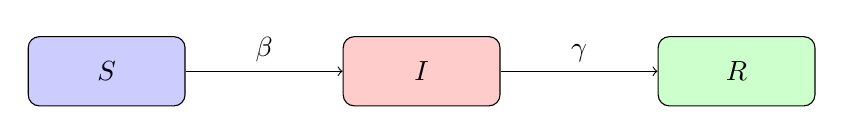
\begin{tikzpicture}
% Susceptible
\path (1.,2.) node [susceptible] (S)  {$S$};
% Infectious
\path (5.,2.) node [infectious] (I) {$I$};
 % Removed
\path (9.,2.) node [removed] (R) {$R$};
% arrows
\draw [->] (I) -- node [above] {$\mathbf{\gamma}$} (R.west);
\draw [->] (S) -- node [above] {$\mathbf{\beta}$} (I.west);
\end{tikzpicture}}
    \caption{\textbf{Model A:} susceptible – infectious – recovered (SIR) modeling framework for homogeneously mixed population.}\label{F:homo}
\end{figure}

\begin{figure}[thpb]
    \resizebox{0.46\textwidth}{!}{% We need layers to draw the block diagram
\pgfdeclarelayer{background}
\pgfdeclarelayer{foreground}
\pgfsetlayers{background,main,foreground}

\begin{tikzpicture}
% Susceptible
\path (1.,2.) node [susceptible] (S1)  {$S_{\mathrm{1}}$};
\path (1.,0.) node [susceptible] (S2)  {$S_{\mathrm{2}}$};
% Infectious
\path (5.,2.) node [infectious] (I1) {$I_1$};
\path (5.,0.) node [infectious] (I2) {$I_{2}$};
 % Removed
\path (9.,2.) node [removed] (R1) {$R_1$};
\path (9.,0.) node [removed] (R2) {$R_2$};
% Arrows
\draw [->] (I1) -- node [above] {$\mathbf{\gamma}$} (R1.west);
\draw [->] (I2) -- node [above] {$\mathbf{\gamma}$} (R2.west);
\draw [->] (S1) -- node [above] {$\mathbf{\beta}_1$} (I1.west);
\draw [->] (S2) -- node [above] {$\mathbf{\beta}_2$} (I2.west);

\begin{pgfonlayer}{background}
\path[fill=blue!10,rounded corners] (-0.5,-0.8) rectangle (2.5,2.8);
\path[fill=red!10,rounded corners] (3.5,-0.8) rectangle (6.5,2.8);
\path[fill=green!10,rounded corners] (7.5,-0.8) rectangle (10.5,2.8);
\path[rounded corners, draw=black!50, dashed] (-0.5,1.2) rectangle (10.5,2.8);
\path[rounded corners, draw=black!50, dashed] (-0.5,-0.8) rectangle (10.5,0.8);
\end{pgfonlayer}
\end{tikzpicture}
}
    \caption{\textbf{Model B/C:} susceptible – infectious – recovered (SIR) modeling framework for age-dependent mixed population.}\label{F:het}
\end{figure}

\subsection{Assumptions}
We propose a two compartment model whose compartments correspond to contact frequency; either high or low. We classify high contact individuals as school-age individuals who are younger than nineteen and low contact individuals as individuals who are older than nineteen. According to census data, the initial proportion of the population in the high contact compartment is 21.3\% \cite{statsCanada}. We will assume that once classified, individuals remain in their respective compartments for the duration of the Influenza epidemic and that in each compartment, everyone is equally susceptible and equally infectious. Further, we assume the recovery rate is the same for all individuals.

Our model does not take into account diseased induced mortality (or naturally induced mortality) because it has a negligible population-level effect for influenza \cite{InfluenzaPeriod}.
Furthermore, since we are only interested in the behavior of a single epidemic, individuals are assumed to acquire permanent immunity during a single epidemic.
Evidence for transmission of influenza by infected individuals before they show symptoms is weak \cite{InfluenzaLatentPeriod}. Thus, the latent period is neglected by our proposed framework. Finally, our model does not consider the possible effects of vaccination against Influenza. 
%\alex{The following assumptions will be made in order to create a model. Firstly, we will assume that the population size is fixed, which indicates that there will be no births and no death due to natural causes or Influenza. There will be two compartments of individuals; high contact individuals and low contact individuals. We will assume that individuals stay in their respective compartments during the duration of the Influenza epidemic and that in each compartment, everyone is equally susceptible and equally infectious. However, the recovery rate for high contact individuals is the same for low contact individuals. We classify high contact individuals as individuals who younger than nineteen (as they are in school) and low contact individuals as individuals who are older than nineteen (as they are not in school). Therefore, the initial proportion of the population in the high contact compartment is 21.3\% as 21.3\% of Canada's population is under 19 \cite{statsCanada}. In addition, since we are only interested in the behaviors of a single epidemic, we assume individuals acquire permanent immunity during a single epidemic. Based of the findings from Patrozou \& Mermel, the latent period needs not be included in our model \cite{InfluenzaLatentPeriod}. Finally, the last assumption being made is that no one is vaccinated against Influenza.}

\subsection{Framework}

A homogeneously-mixed population can be modeled, using the framework shown in \fref{homo}, by the system of non-linear ordinary differential equations \eqref{eq:homo}, where $\beta$ is the transmission rate, $\gamma$ is the infection rate and $S$, $I$ and $R$ is the proportion of the population susceptible, infected and recovered from Influenza respectively. 
\begin{subequations}\label{eq:homo}
\begin{eqnarray}
\frac{dS}{dt} =& -\beta S I \label{eq:SIRdSdt}\\
\frac{dI}{dt} =& \beta S I - \gamma I \label{eq:SIRdIdt}\\
\frac{dR}{dt} =& \gamma I \label{eq:SIRdRdt}
\end{eqnarray}
\end{subequations}

A heterogeneously-mixed population can be modeled, using the framework shown in \fref{het}, by the system of non-linear ordinary differential equations \eqref{eq:het}, where $\beta_1$ is the transmission rate for the \emph{high interaction} compartment, $\beta_2$ is the transmission rate for the \emph{low interaction} compartment. One should note that $\beta_1 = \beta\cdot\alpha_1$, where $\alpha_1$ is the \textit{transmission interactivity factor} for the high interaction compartment and $\beta_2 = \beta\cdot\alpha_2$, where $\beta_2$ is the \textit{transmission interactivity factor} for the low interaction compartment. $\alpha_1$ and $\alpha_2$ is the factor by which the probability of infection increases in the the high interaction compartment and low interaction compartment respectively. $S_1$, $I_1$ and $R_1$ is the proportion of individuals in the high interaction compartment that are susceptible, infected and recovered respectively. Similarly, $S_2$, $I_2$ and $R_2$ is the proportion of individuals in the low interaction compartment that are susceptible, infected and recovered respectively.

\begin{subequations}\label{eq:het}
\begin{eqnarray}
\frac{dS_1}{dt} =& -\beta_1 S_1 (I_1 + I_2) \label{eq:SIRdS1dt}\\
\frac{dS_2}{dt} =& -\beta_2 S_2 (I_1 + I_2)\label{eq:SIRdS2dt}\\
\frac{dI_1}{dt} =& \beta_1 S_1 (I_1 + I_2) - \gamma I_1\label{eq:SIRdI1dt}\\
\frac{dI_2}{dt} =& \beta_2 S_2 (I_1 + I_2) - \gamma I_2 \label{eq:SIRdI2dt}\\
\frac{dR_1}{dt} =& \gamma I_1 \label{eq:SIR_het_dr} \label{eq:SIRdR1dt}\\
\frac{dR_2}{dt} =& \gamma I_2 \label{eq:SIRdR2dt}
\end{eqnarray}
\end{subequations}
Note that since equations \eqref{eq:SIRdSdt}-\eqref{eq:SIRdIdt} and \eqref{eq:SIRdS1dt}-\eqref{eq:SIRdI2dt} do not depend on the recovered class $R$, equations \eqref{eq:SIRdRdt}, \eqref{eq:SIRdR1dt}, and \eqref{eq:SIRdR2dt} can be ignored.

\subsection{Parameters}

The basic reproduction number $\R_0$ (the average number of secondary cases caused by a given primary case in a wholly susceptible population) is given by:
\begin{equation}\label{eq:Ro}
\R_0=\frac{\beta}{\gamma}
\end{equation}
We know for the flu that $\R_0 = 1.8$ \cite{reproductiveno.influenza}, the mean infectious period is $\gamma^{-1} = 3.33$ \cite{reproductiveno.influenza} which indicates that 
$\beta = 0.54$ (for the homogeneously-mixed model).


\section{RESULTS}


\begin{figure}[thpb]
\centering
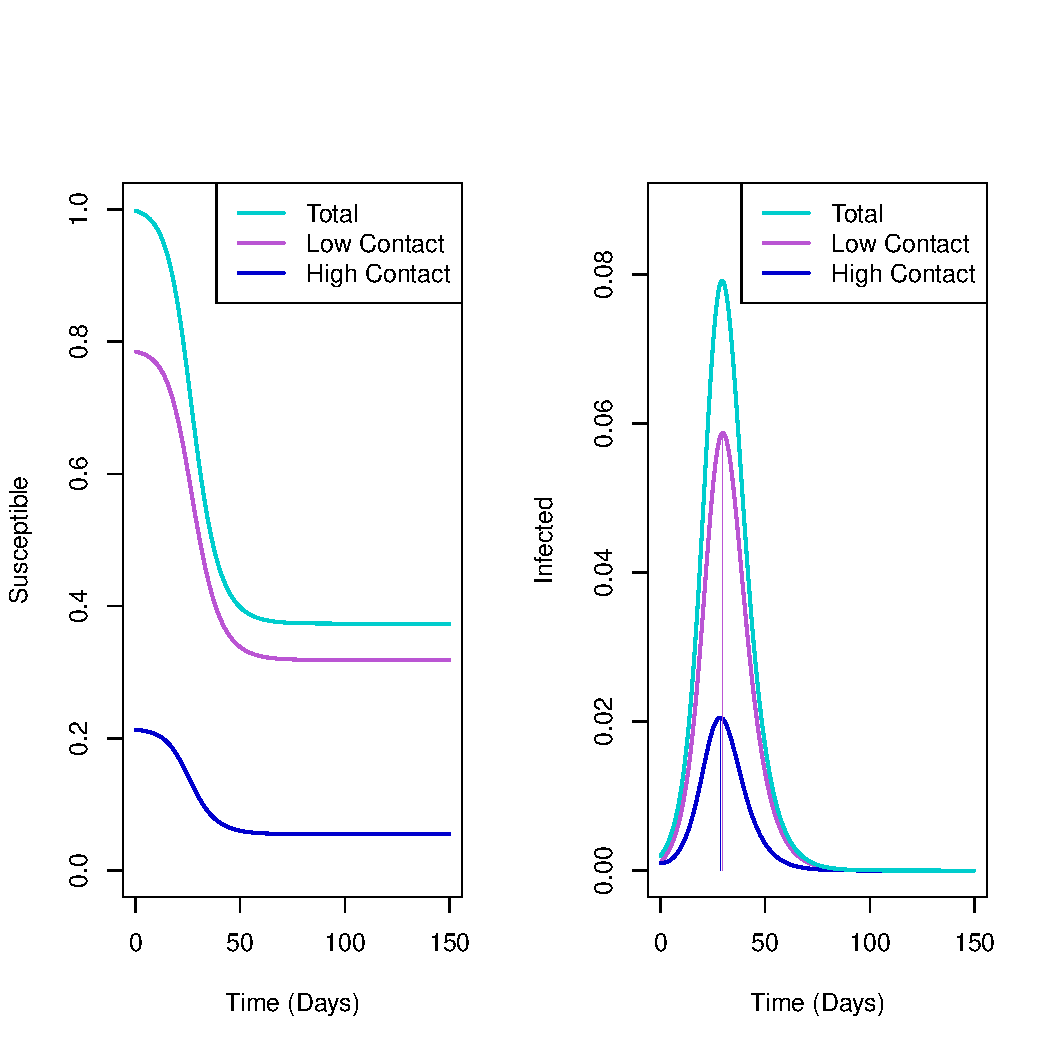
\includegraphics[scale = 0.44]{figure/R_B-1.pdf}
\caption{The parameters that produced the above graphs are $\beta = 0.54$, $\alpha_1 = 1.2$, $\alpha_2 = 0.8$ and $\gamma = 0.3$. A higher transmission rate seems to imply that the peak of the epidemic will occur earlier and the epidemic will die out quicker. The final size can also be determined from the graph on the left. However, this will be discussed later.}\label{F:contact}
%\vskip -15pt
\end{figure}

\begin{figure}[thpb]
\centering
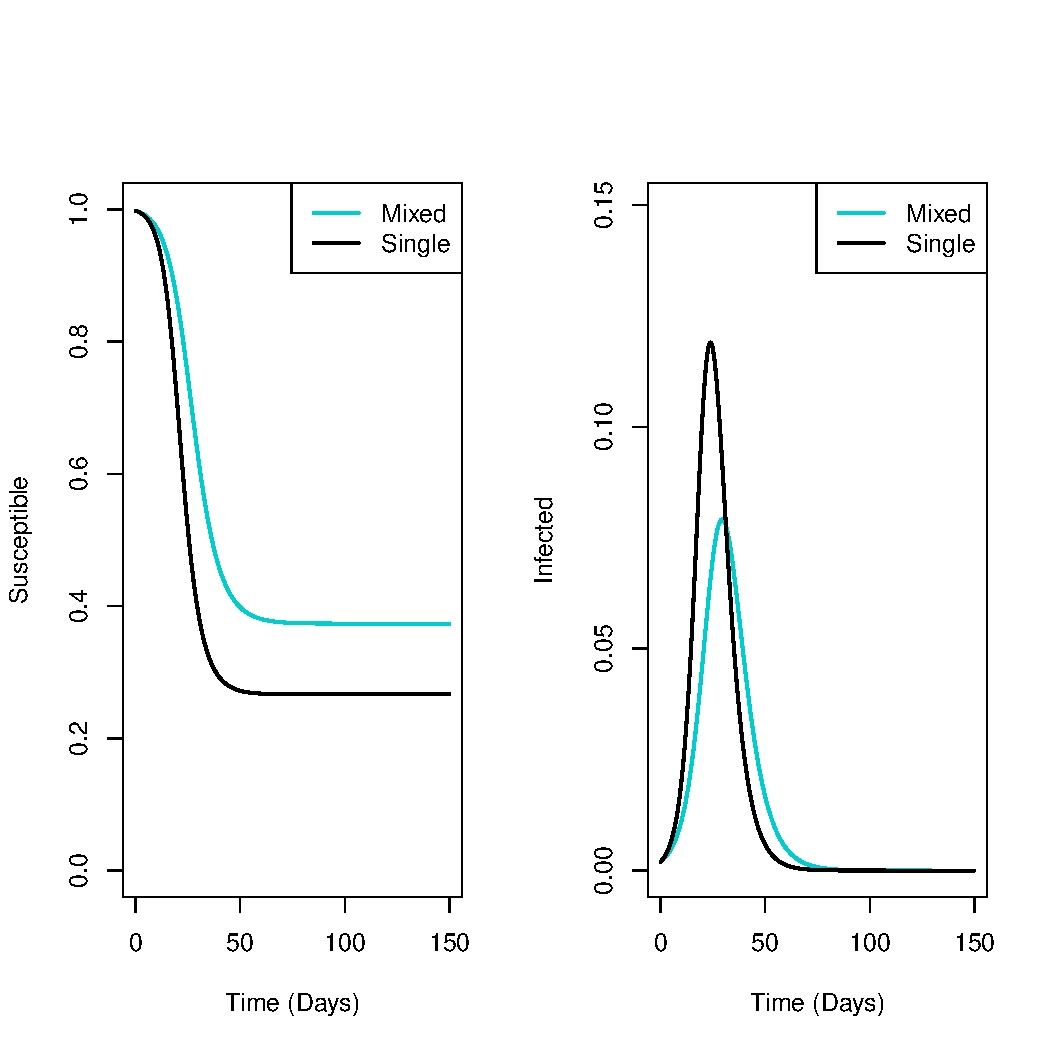
\includegraphics[scale = 0.44]{figure/R_AB-1.pdf}
\caption{The value of $\beta$ for Model A is $0.54$. The parameters used for Model B are the same parameters used to generate \ref{F:contact}. Model B has a much better outcome compared with the homogeneously-mixed model as the peak of the epidemic contains approximately half the of the size. It's also evident that the final size of the epidemic for Model B is much less than the final size for Model A.}\label{F:Homovshetero}
\end{figure}



\begin{figure}[thpb]
\centering
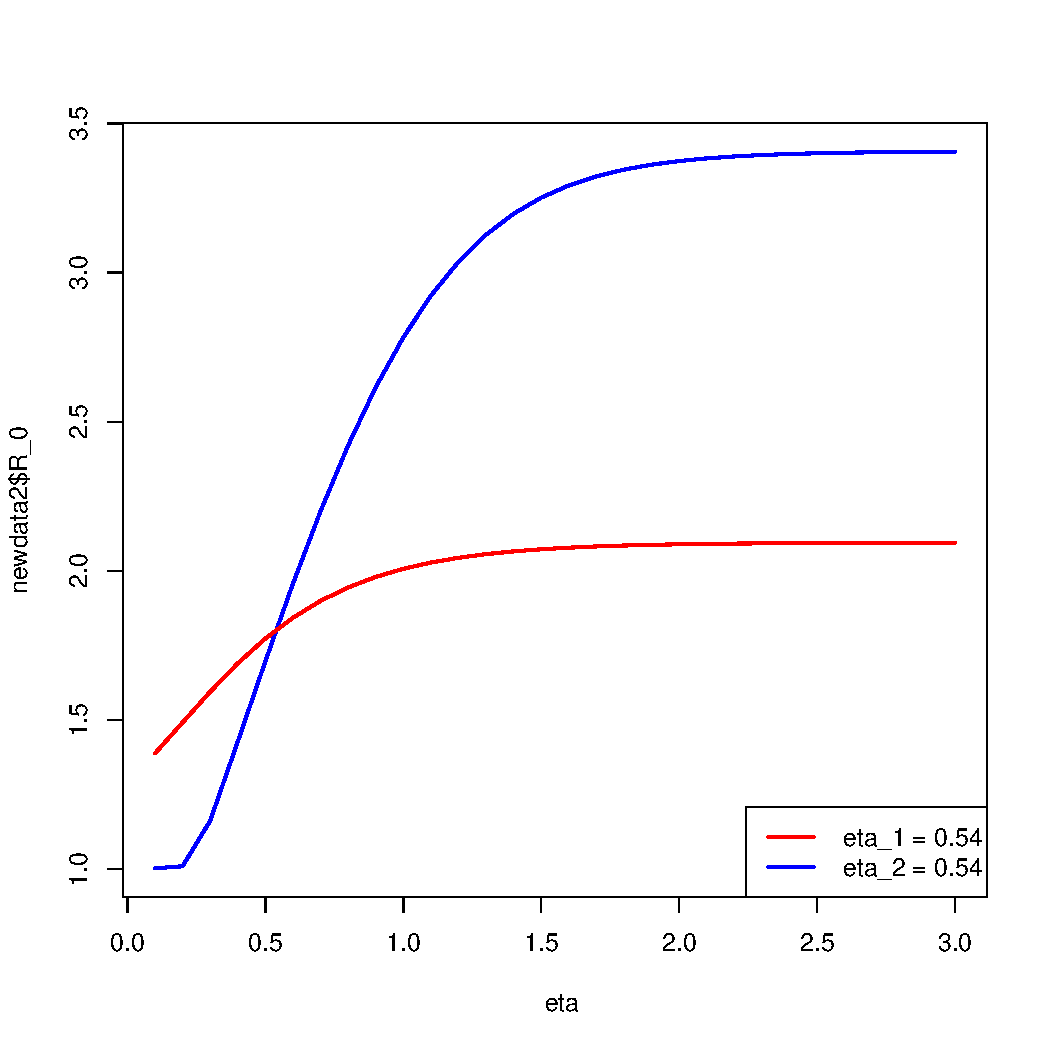
\includegraphics[scale = 0.44]{figure/R_beta-1.pdf}
\caption{Fixing $\beta_2 = 0.54$ and varying $\beta_1$ gives the blue line and fixing $\beta_1 = 0.54$ and varying $\beta_2$ gives the red line. Using \eqref{Eq:Z}, one can find the estimated value of $\R_0$ from the final size as a function of the $\beta$ we are varying.}\label{F:R_0}
\end{figure}

\begin{figure}[thpb]
\centering
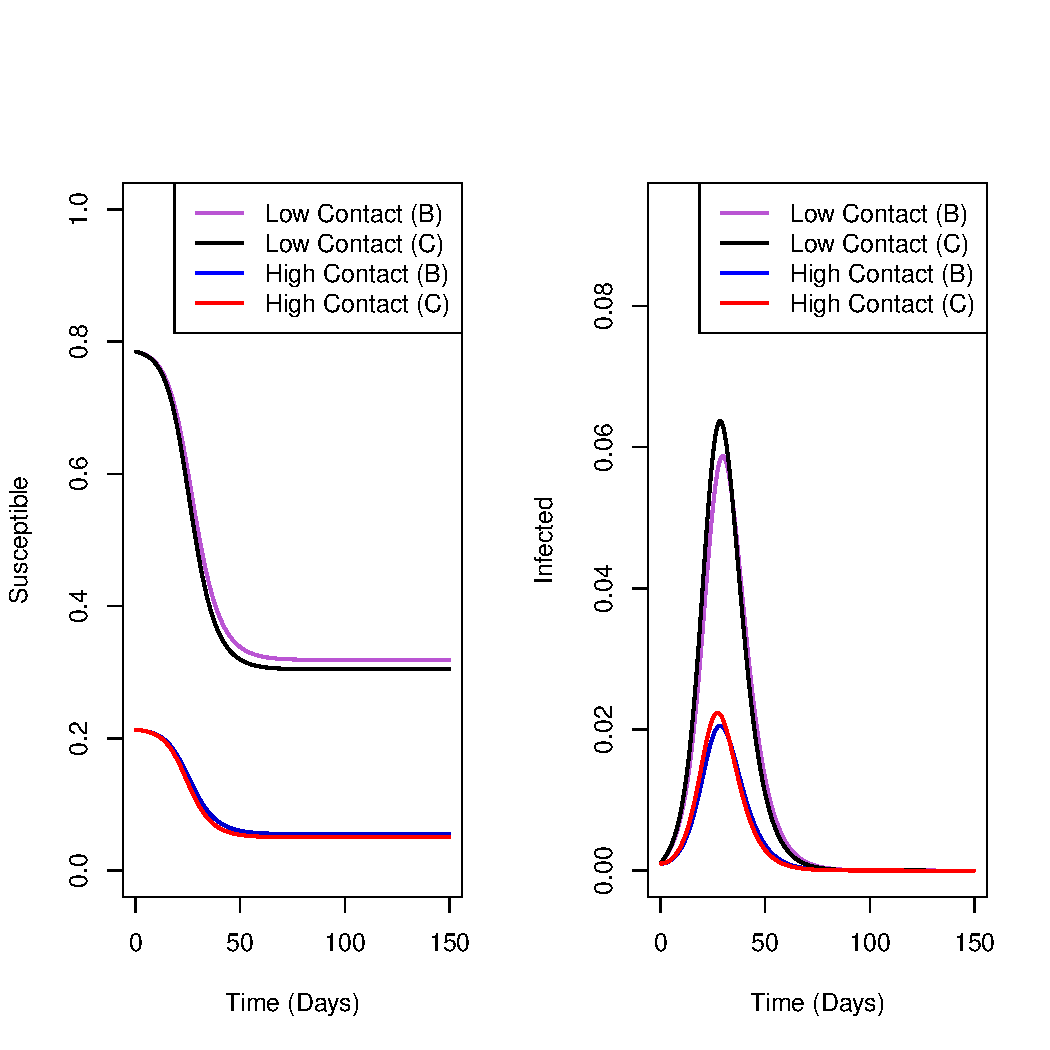
\includegraphics[scale = 0.44]{figure/R_BC-1.pdf}
\caption{Provides a comparison for Model B and Model C. The figure on the left shows the proportion of susceptible individuals at a given time for the low and high contact individuals in Model B and Model C. The figure on the right shows the proportion of infected individuals at a given time for the low and high contact individuals in Model B and Model C.}\label{F:ModelC}
\end{figure}

\fref{contact} shows the percentage of individuals who are susceptible and infected at a given time for the two compartments, and the total population, using the framework shown in \fref{het}. Initially, $S_1 = 0.213$ and $S_2 = 0.785$. After the epidemic occurred, the proportion of susceptibles remaining was $S_1 = 0.0550$ and $S_2 = 0.3185$. This means that the susceptible class with a higher interaction rate had 74\% of their population get Influenza and the susceptible class with a lower transmission rate had 59\% of their population get Influenza over 150 days. Clearly, and logically, a higher interaction rate will lead to a higher probability of inheriting Influenza. Also shown on \fref{contact} is when the peak prevalence occurs. For the high and low interaction compartment, the peak prevalence is 0.0205 at 28 days and 0.0587 at 29 days respectively. This implies a higher transmission rate will generate an earlier peak prevalence. 

More interestingly, \fref{Homovshetero} provides a comparison of Models A and B. The percentage of individuals who are susceptible at a given time varies quite drastically between the two models, particularly at later times. Given $\beta = 0.54$, $\alpha_1 = 1.2$, $\alpha_2 = 0.8$ and $\gamma = 0.3$, our calculations predict that the maximum percentage of the population infected at a given time is 11.90\%, using Model A, and 7.91\%, using Model B. In addition, the estimated final size of the epidemic is 0.7335 $(1-0.2665)$, according to Model A, and is 0.6265 $(1 - 0.3735)$, according to Model B. 

Using the final size calculated from this simulation, one can find the value of $\R_0$ from the final size using \eqref{Eq:Z}, which was derived by Kermack and McKendrick in 1927 \cite{Kermack700}. Ma \& Earn, 2006 \cite{Ma2006} showed that \eqref{Eq:Z} can be used for more realistic models, and therefore, we will be using it for our analysis.
\begin{equation}\label{Eq:Z}
Z = 1 - e^{-\R_0 Z}
\end{equation}

\fref{R_0} gives a comparison of the transmission rate for a certain compartment by fixing the transmission rate of the other compartment by 0.54. From this graph, it's evident that $\beta_1$ is mainly driving the dynamics of this model as the resulting $\R_0$ at a high $\beta$ is large when we fix $\beta_2$. It's interesting to note that even at a certain value of $\beta$, the value of $\R_0$ does not change with an increasing $\beta$.

Model B provides a contact-structured model that allows us to separate the population into two classes based upon the individual's interactivity. These dynamics of Model B differ greatly from the dynamics of Model A, which seems to indicate that including this contact-structure is essential. To test this hypothesis, one would need to compare these models against Influenza epidemic data, with the initial conditions and parameters reflecting the population being studied accurately. 
\\

Earn \textit{et al.} discuss that their model incorporating the use of antipyretics should also consider the effect of age \cite{Earn_fever}. In our case, we will consider antipyretic use in conjunction with Model B, which gives us Model C. Model C can be represented with the same set of equations as Model B \eqref{eq:het}, except $\beta_1 = \beta \cdot \alpha_1 \cdot f_1$ and $\beta_2 = \beta \cdot \alpha_2 \cdot f_2$, where $f_1$ and $f_2$ is the increased overall increase in the transmission rate due to antipyretics, which is called the \textit{population transmission enhancement factor}. Earn \textit{et al.} derived \eqref{Eq:f}, where $p$ is the proportion of individuals taking antipyretics that have Influenza and  $f_i$ is the increase in infectivity for an individual, which is called the \textit{individual transmission enhancement factor}.

\begin{equation}\label{Eq:f}
f_p = 1 + p(f_i - 1)
\end{equation}

Earn \textit{et al.} estimate that $f_i = 1.06$ and using assumptions mentioned in the paper, we will conclude that $p = 0.603$, which gives $f_p = 1.03618$ for the high interactivity class and $p=0.325$, which gives $f_p = 1.0195$ and for the low interactivity class.

Figure \ref{F:ModelC} gives a comparison for Models B and C. Comparing the two models, one can see that the models do not have as much of a drastic difference from each other, compared with the difference between Model A and Model B. 

\alex{maximum infected for Model C is 0.02234989 for high contact 0.06368935 for low contact, estimated final size 0.698 (1-0.3043428) - low contact 
0.05023666 - high contact}

\alex{estimated final size 0.6454 (1-0.3545795)}

\section{CONCLUSIONS}
-Elaborate on the importance of the work or suggest applications and extensions. 
 
 If possible, see the effects of a three level age-structured model.

\addtolength{\textheight}{-12cm}   % This command serves to balance the column lengths

%%%%%%%%%%%%%%%%%%%%%%%%%%%%%%%%%%%%%%%%%%%%%%%%%%%%%%%%%%%%%%%%%%%%%%%%%%%%%%%%
%\section*{APPENDIX}
%(If we end up needing one)
%%%%%%%%%%%%%%%%%%%%%%%%%%%%%%%%%%%%%%%%%%%%%%%%%%%%%%%%%%%%%%%%%%%%%%%%%%%%%%%%

\bibliographystyle{vancouver}
\bibliography{TheFourHumours}

\end{document}

